\documentclass[conference]{IEEEtran}
\usepackage[letterpaper,left=0.75in,right=0.75in,top=1in,bottom=0.75in]{geometry}
\usepackage{amsmath,amssymb}
\usepackage{graphicx}
\usepackage{booktabs}
\usepackage{array}
\usepackage{multirow}
\usepackage{cite}
\usepackage{xcolor}
\usepackage{colortbl}
\usepackage{algorithm}
\usepackage{algpseudocode}
\usepackage{tikz}
\usetikzlibrary{arrows.meta,positioning}

\newcommand{\cmark}{\textbf{pass}}
% Numeric tables stay unfilled; plots carry the visual encoding.
\definecolor{goodrow}{gray}{1.0}
\definecolor{badrow}{gray}{1.0}
\definecolor{hdr}{gray}{1.0}
\definecolor{boxA}{RGB}{252,238,225}
\definecolor{boxB}{RGB}{230,241,251}
\definecolor{boxC}{RGB}{232,246,236}
\definecolor{accentOrange}{RGB}{217,121,65}
\definecolor{accentBlue}{RGB}{42,111,187}
\definecolor{accentGray}{RGB}{89,99,110}

\begin{document}

\title{AGCD: Auditing Failure-Driven Policy\\
Improvement in World--Action Models}

\author{\IEEEauthorblockN{Anonymous Authors}
\IEEEauthorblockA{Paper \#ICRA2027}
}

\maketitle


\begin{abstract}
Action-conditioned manipulation predictors can score candidate actions for the
wrong reason. Perturbing expert actions and retaining terminal outcomes injects
an \textit{action-amplitude shortcut}: magnitude encodes success while geometry
is ignored. We release \textbf{AGCD}, an intervention test that audits this
leak, collects action-matched/geometry-varied counterfactuals, and verifies the
same predictor by closed-loop selection. Action-L2 reaches AUROC~$0.90$ on the
victim recipe but collapses to~$0.50$ under paired geometry. The same MiniWAM
trained on perturbation versus paired data yields paired AUROC~$0.50$ vs~$0.99$
and closed-loop success~$0.29$ vs~$0.96$ (gap~$0.67$, 95\% CI~$[0.52,0.79]$);
FACT/RGB/DINOv2 variants retain gaps of~$0.62$--$0.65$. Distilling
evaluator feedback into the same policy gives success~$0.296$ vs~$0.976$ for
confounded vs paired feedback, with no evaluator query at test time. Physics-based
PyBullet push and carry-release preserve gains of~$0.722$ and~$0.651$; in the
latter, confounded feedback avoids drops yet sends $65.1\%$ of trials to wrong
targets. With frozen DINOv2 input and an independently BC-initialized policy,
paired-feedback success remains $0.84$--$0.96$ under noise, blur, crop,
occlusion, and color shifts, improving over no update by $0.24$--$0.30$. Fix the
feedback contract before using failures to improve a policy.
Generators, baselines, and audit gates: \texttt{https://anonymous.4open.science/r/icra-8056/}.
\end{abstract}

\begin{IEEEkeywords}
world model, counterfactual, shortcut learning, diagnostic suite, manipulation
\end{IEEEkeywords}



\section{Introduction}
\label{sec:intro}

When a world-action model (WAM) ranks candidate actions by predicted progress or
risk~\cite{ha2018recurrent,hafner2025mastering,fact2026}, the ranking is useful
only if it reflects \emph{action--geometry interaction}. If the score is a
disguised function of action magnitude, selective execution is internally
consistent and physically empty.

\paragraph{The closed-loop question.}
AGCD asks whether holding the action fixed while changing visible geometry
changes the predictor's decision in the same direction as the rollout. Thus the
paper follows one chain: confounded collection, ranking failure, paired
collection, and ranking recovery on unseen layouts.

That failure mode is not hypothetical as a compositional risk. Recovery
pipelines perturb demonstrations~\cite{flare2026}, while benchmark collectors
expose terminal task outcomes~\cite{rlbench2019}; outcome heads separately
train on progress/value targets~\cite{fact2026}. Connecting these ingredients---
supervising an outcome head with expert-perturbation success---creates an
\textit{action-amplitude shortcut}: large perturbations fail, small ones succeed,
so $\|a-a_{\mathrm{nom}}\|$ predicts~$y$ without consulting geometry.

\paragraph{Positioning.}
We study a \emph{compositional} risk, not a smear of named checkpoints. FLARE's
perturbations are for recovery; FACT's value heads are for failure-aware
futures; neither paper advocates the dangerous wiring
(Table~\ref{tab:recipe}). The risk appears when
``perturb demos $\rightarrow$ keep success $\rightarrow$ train value'' becomes
the default next step---a wiring that is easy to invent once both ingredients
exist in the ecosystem. AGCD makes that step falsifiable \emph{before} it
scales: detect the leak, ship an intentional victim, and show that changing the
\emph{collection protocol} (not the loss) restores decision quality.

\begin{figure}[!t]
\centering
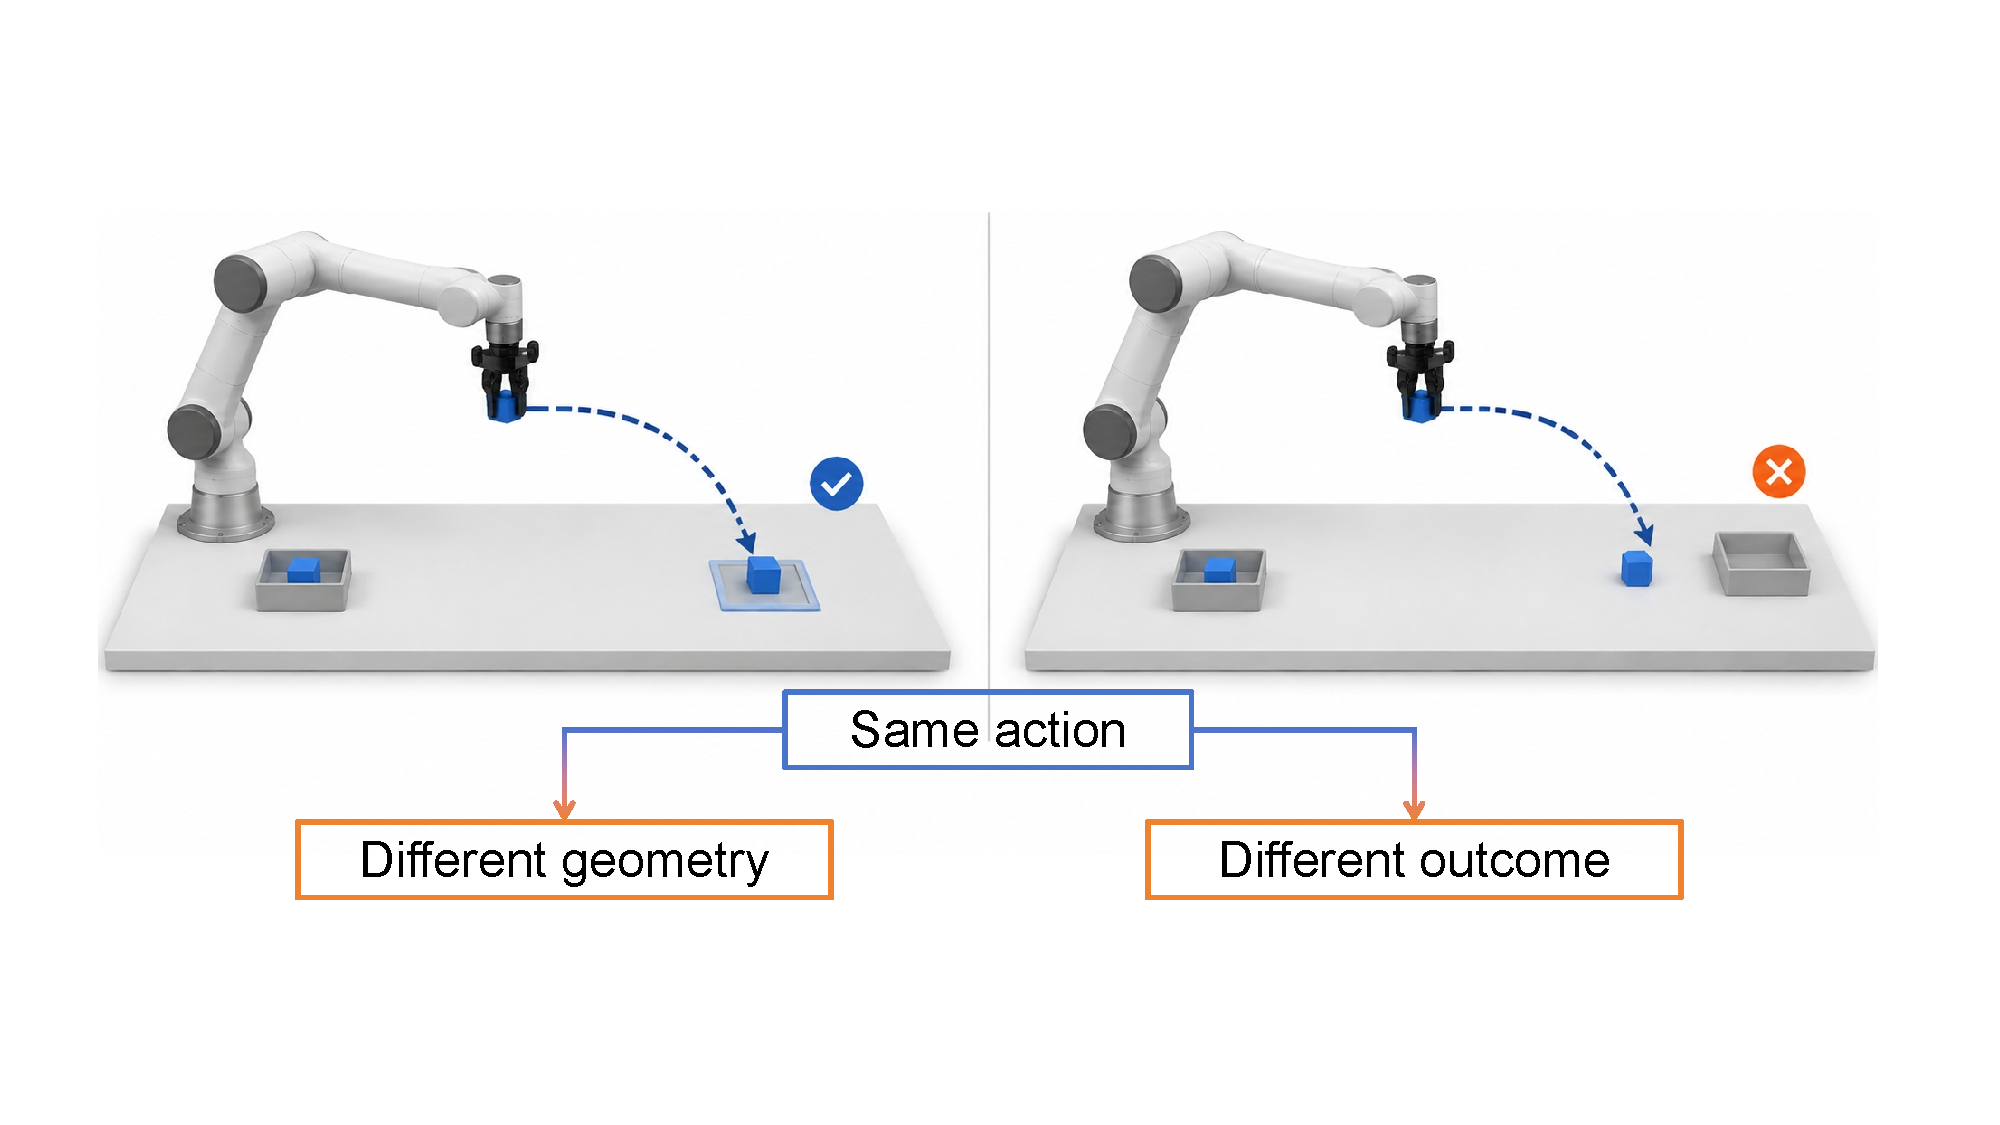
\includegraphics[width=\columnwidth]{figures/fig1.pdf}
\caption{\textbf{Motivating observation.} The same action yields different
outcomes when target geometry changes. AGCD tests whether a predictor uses this
interaction rather than action amplitude.}
\label{fig:teaser}
\end{figure}

\paragraph{Concrete failure.}
On a fixed pick-place layout, replay the expert with joint noise
$\sigma\in\{0.02,0.04,0.06,0.08\}$. Large-$\sigma$ episodes drop; small-$\sigma$
episodes succeed. An outcome head can ignore seats and still post high AUROC by
reading amplitude. Now hold the \emph{same} action and move the target:
amplitude is constant, yet success flips with geometry. Any model that learned
the first cue fails the second---and closed-loop $\arg\max$ over matched
directions collapses onto the min-L2 heuristic. The diagnostic question is
whether changing only how labels are collected restores geometry-aware ranking.

\paragraph{Contributions.}
\begin{enumerate}
\item \textbf{Intervention test:} an A/B audit identifies whether an outcome
predictor can solve the recipe from action amplitude alone.
\item \textbf{Paired protocol:} an action-matched factorial collector removes
that cue while preserving action--geometry interaction.
\item \textbf{Learning closure:} the same heads and candidates are evaluated
offline, in closed-loop selection, and through evaluator-guided policy updates
whose held-out execution no longer queries the evaluator.
\end{enumerate}



\section{Related Work}
\label{sec:related}

\begin{table*}[t]
\centering
\caption{\textbf{Recipe audit} of the dangerous chain
(perturb expert $\rightarrow$ keep success $\rightarrow$ train outcome/value).
Cells summarize the cited work; the generic collector row is a possible
composition, not a claim that any released system trains this full chain.}
\label{tab:recipe}
\setlength{\tabcolsep}{3pt}
\begin{tabular*}{\textwidth}{@{\extracolsep{\fill}}lcccc@{}}
\toprule
\rowcolor{hdr}
Work
  & Expert pert.?
  & Success as label?
  & Outcome/value head?
  & Full chain? \\
\midrule
FLARE \cite{flare2026}
  & yes (Retry bridges)
  & no (policy target)
  & no
  & no \\
FACT \cite{fact2026}
  & no (policy fails)
  & yes (progress/value)
  & yes
  & no \\
CoCo \cite{coco2026}
  & CF for consistency
  & n/a
  & no
  & no \\
ACT-Bench \cite{actbench2024}
  & eval only
  & no
  & metrics
  & no \\
Validate the Dream \cite{validate2026}
  & n/a
  & n/a
  & accreditation
  & no \\
Generic RLBench-style collector
  & yes (possible)
  & yes (terminal)
  & optional next step
  & \emph{not inherent} \\
\midrule
\rowcolor{goodrow}
\textbf{AGCD victim (ours)}
  & \textbf{yes}
  & \textbf{yes}
  & \textbf{yes}
  & \textbf{yes (intentional)} \\
\bottomrule
\end{tabular*}
\end{table*}

\paragraph{Action-conditioned prediction.}
Action-conditioned video prediction established the basic premise that a robot
can learn physical consequences directly from interaction videos
\cite{finn2016video}; visual foresight then connected those predictions to
model-predictive control on a real robot~\cite{finn2017foresight}. Latent
world-model planning provides the corresponding compact-state formulation
\cite{hafner2019planet}.
WAMs couple action generation with future prediction or consequence
scoring~\cite{fact2026,motus2_2026,gwm2026,vggtworld2026,vggtomega2026,vggt4d2025}.
PointWorld predicts full-scene 3-D point flow conditioned on robot point
flow~\cite{pointworld2026}; Diffusion Policy illustrates why modern policies
naturally emit multi-step candidate chunks rather than isolated controls
\cite{chi2023diffusion}. These developments make counterfactual ranking useful,
but also make a scalar property of the candidate chunk available to every
downstream head. ACT-Bench and Validate the Dream test action fidelity and
accreditation~\cite{actbench2024,validate2026}; CoCo targets visual inertia with
a consistency objective~\cite{coco2026}. AGCD instead audits whether the
\emph{outcome labels themselves} reveal the answer through action amplitude.

\paragraph{Failure data and causal confusion.}
Table~\ref{tab:recipe} audits a compositional risk rather than naming a guilty
checkpoint. FLARE perturbs demonstrations for recovery~\cite{flare2026}, but
does not train an outcome head on the success of those perturbations. FACT
trains progress/value on policy failures~\cite{fact2026}, not on
expert-action perturbations. Classical DAgger changes the visited-state
distribution by online aggregation~\cite{ross2011dagger}; causal confusion in
imitation learning shows that predictive features can still identify the wrong
causal mechanism under intervention~\cite{dehaan2019causal}. Our failure is a
concrete label-construction instance: perturbation scale jointly changes both
the action and its probability of success. Shortcut learning and invariant
risk minimization motivate environment interventions, but do not specify the
manipulation data crossing needed here~\cite{geirhos2020shortcut,arjovsky2019irm}.
Motus2 routes failed and suboptimal interactions to simulation/value learning
and feeds value estimates back into planning and policy updates
\cite{motus2_2026}. AGCD asks the complementary upstream question: whether the
failure recipe makes that feedback identifiable from action--geometry
interaction before it is allowed to update the policy.

\paragraph{Robot data and decision confidence.}
RoboNet, BridgeData V2, DROID, and Open X-Embodiment provide broad robot
experience across platforms and scenes
\cite{dasari2020robonet,bridgedata2023,khazatsky2024droid,openx2024}; robomimic
systematizes offline demonstration evaluation~\cite{mandlekar2022robomimic},
while LIBERO and CALVIN stress task transfer and long-horizon control
\cite{liu2023libero,mees2022calvin}. Scale and
diversity do not by themselves supply outcome-balanced, same-action/different-
geometry interventions; Sec.~\ref{sec:public_audit} tests this boundary rather
than treating demonstrations as a failure benchmark. Calibration and selective
prediction make a valid score operational~\cite{guo2017calibration,
geifman2019selective}; conformal risk control can additionally bound a chosen
monotone loss on held-out calibration data~\cite{angelopoulos2024crc}. However,
temperature scaling preserves ranking and rejection
cannot repair a target whose shortcut is already encoded in the labels. AGCD is
therefore upstream of calibration: first establish that geometry changes the
ranking, then calibrate or abstain.

\section{The AGCD Diagnostic}
\label{sec:method}

\begin{figure*}[!t]
\centering
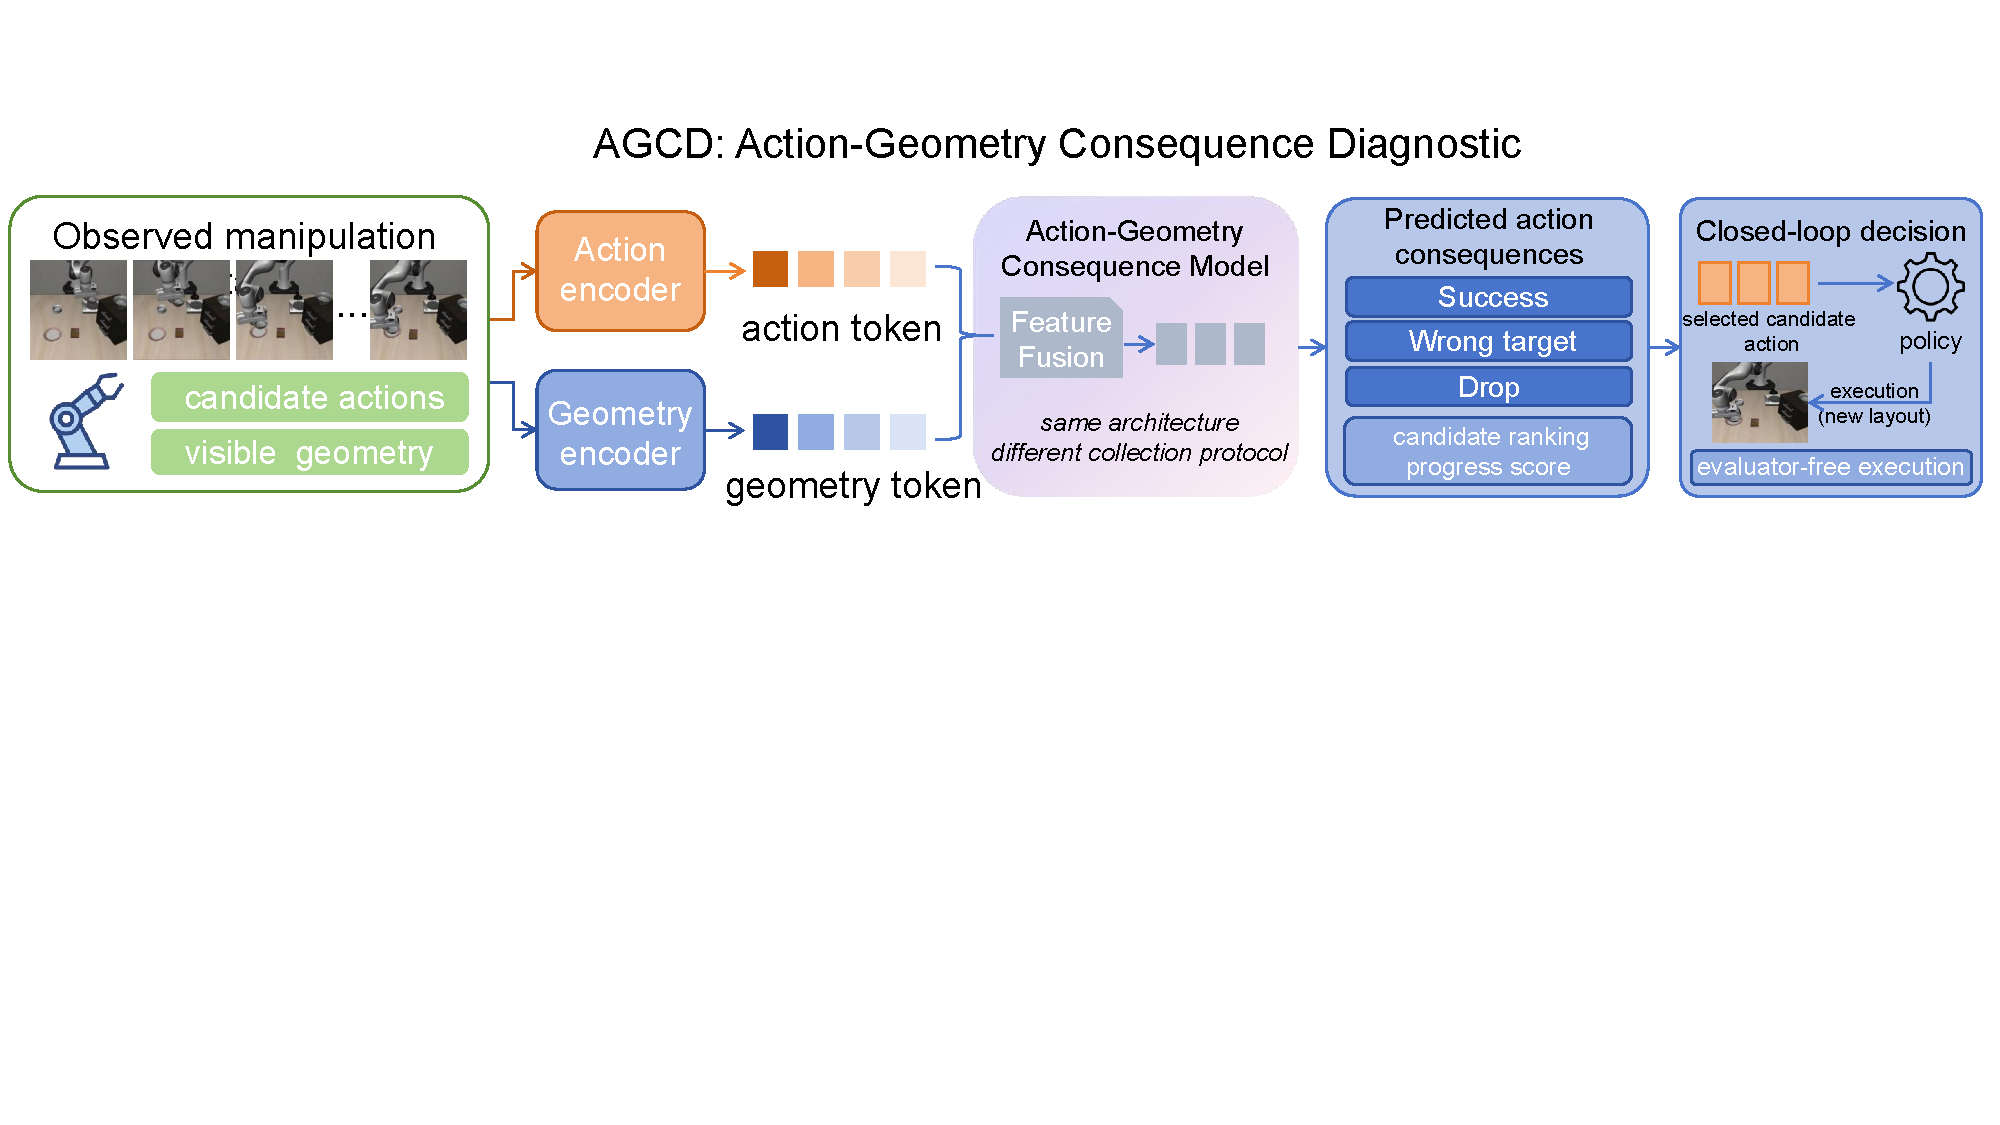
\includegraphics[width=0.98\textwidth]{figures/fig2.pdf}
\caption{\textbf{AGCD method overview.} Observed manipulation states, visible
geometry, and candidate actions are encoded and fused to predict action
consequences (success, wrong target, or drop), rank candidates, and make a
closed-loop execute-or-reject decision.}
\label{fig:pipeline}
\end{figure*}

\subsection{Threat model}
Let $a$ be an action chunk, $g$ scene geometry, and $y\in\{0,1\}$ terminal
success. A consequence predictor $f(a,g)$ is useful for selective execution only
if its ranking depends on the interaction $(a,g)$, not on a scalar summary of
$a$ alone. Expert-perturbation CF draws
$\tilde a=a_{\mathrm{nom}}+\epsilon$ on fixed~$g$ and labels by rollout success.
Write $s=\|\tilde a-a_{\mathrm{nom}}\|$ (or mean per-step L2). If
$\mathrm{AUROC}(s\rightarrow y)$ is high on the training recipe while
$\mathrm{AUROC}(s\rightarrow y)\approx 0.5$ under paired geometry, then labels
are not pure action--geometry interactions: $y\not\perp g\mid s$ fails in the
direction that matters for ranking. Empirical risk minimization may ignore~$g$
and still look strong in-domain.

Noise for coverage is fine. Using noise-induced success as outcome supervision
\emph{without} amplitude control is the threat (Fig.~\ref{fig:pipeline}).
Paired-geometry collection is the complementary intervention: hold $a$ fixed
(or scalar-matched) and vary $\{g_k\}$ so that $s$ carries no label information.

\subsection{Identification by factorial crossing}
The minimal paired unit is not a positive/negative trajectory pair; it is a
crossing of action identity and geometry. Let $A=\{a_i\}_{i=1}^{m}$ be
candidate directions and $G=\{g_j\}_{j=1}^{n}$ be layouts. We execute every
cell $(a_i,g_j)$ and obtain the rollout label
\begin{equation}
 y_{ij}=\mathbb{1}\!\left[\text{task succeeds after executing }a_i
 \text{ in }g_j\right].
 \label{eq:factor}
\end{equation}
The design is valid only when neither row nor column identity determines the
label: each action succeeds and fails across layouts, and each layout succeeds
and fails across actions. In the three-way controlled task this yields a
permuted diagonal pattern: matching direction and target succeeds; the other
cells become wrong-target or drop. This is stronger than swapping one target
under one fixed action, where geometry identity alone would reveal the label.

\paragraph{Why the amplitude probe must fail on valid pairs.}
Let $m(a)$ collect all scalar action summaries accessible to a shortcut:
mean/max step L2, path length, peak speed, and gripper-transition count. If the
crossing is balanced such that
$p(m(a)\mid y{=}1)=p(m(a)\mid y{=}0)$, any score measurable only from $m(a)$
has AUROC $0.5$ in expectation. This is not a claim that action is irrelevant;
action \emph{direction} is essential through its interaction with geometry.
It says only that a marginal scalar cannot rank the outcomes. AGCD tests this
condition empirically rather than assuming that equal command length implies
equal robot motion.

\paragraph{What is and is not identified.}
The factorial protocol identifies whether a predictor uses information beyond
the audited action scalars on the support of the crossed layouts. It does not
identify the causal effect of arbitrary actions, guarantee extrapolation beyond
that support, or make simulator labels real. Consequently, we require
layout-disjoint evaluation, action-only and geometry-only controls, and a
closed-loop ranking test. A model passes only when the joint input improves over
both marginals and selects the correct action on unseen layouts.

\subsection{Three probes}
\textbf{Probe A (detect).} Build a confounded set (fixed layout, noise ladder)
and a paired set (fixed amplitude, varied geometry). Report
AUROC$(s\rightarrow y)$ on both, plus transfer of an amplitude head trained on
confounded and tested on paired.

\textbf{Probe B (remove).} Collect paired-geometry CF: hold $a$
element-identical (or scalar-matched across directions) while varying $\{g_k\}$.
Amplitude carries no label information; success requires alignment of $a$
with~$g$.

\textbf{Probe C (decide).} Train the \emph{same} action-conditioned head on each
recipe; evaluate both on a shared paired holdout and closed-loop $\arg\max$ over
three matched directions. We report a small MiniWAM (value + short future) and a
\emph{FACT-style} temporal Transformer: action-conditioned progress sequence +
terminal value + short future (2.3M params), matching FACT's scoring interface
rather than its full video backbone. This is intentional. Reproducing FACT's
pixel world model would conflate video modeling capacity with label leakage; our
question is whether a larger progress/value head still falls for the amplitude
shortcut when only the collection recipe changes. Architecture is not the
claim---the claim is the protocol.

\begin{figure*}[t]
\centering
\IfFileExists{figures/fig_paired_qualitative.pdf}{%
  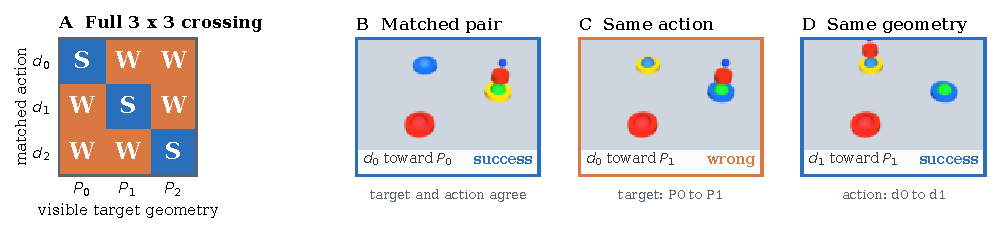
\includegraphics[width=\textwidth,height=3.5cm,keepaspectratio]{figures/fig_paired_qualitative.pdf}%
}{%
  \fbox{\parbox[c][4.2cm][c]{0.96\textwidth}{\centering
  \textbf{Reserved qualitative visualization: paired-geometry matrix}\\[3pt]
  Replace with a $3\!\times\!3$ grid showing the same scalar-matched actions
  across three target layouts. Overlay action direction, target position, final
  object position, and rollout outcome (success / wrong-target / drop).}}
}
\caption{The complete action$\times$geometry crossing from actual MuJoCo
rollouts. Each row holds the candidate action fixed; each column changes only
the visible target geometry. The diagonal is the matched-direction success
pattern; off-diagonal cells are non-success outcomes.}
\label{fig:paired_qualitative}
\end{figure*}

\subsection{Collection contract}
For every decision state, the collector writes a row containing: episode and
layout identifiers; the full action chunk; the action-summary vector $m(a)$;
target and object geometry; terminal object pose; contact-mode outcome; and
success. A paired group is accepted only if (i) all prescribed directions are
present, (ii) action horizons and gripper schedules agree, (iii) scalar spread
is below the configured tolerance, and (iv) at least two outcomes occur. These
checks happen before fitting any predictor. Groups that fail are diagnostics,
not training examples.

Confounded and paired recipes use separate collectors but the same feature
contract, architecture, and layout-level split. Geometry-only and action-only
baselines reuse those indices, so the joint gain cannot come from an easier
split or extra examples.

\paragraph{Reset-free approximation.}
Without exact resets, we retrieve blocks within skill, phase, gripper state,
and a pre-action visual-state neighborhood; impose calipers on all $m(a)$
scalars; and retain geometry-diverse blocks passing balance, overlap, and
outcome-variation checks. These are matched observational evidence unless
geometry was randomized by intervention.

\begin{algorithm}[t]
\caption{AGCD (summary)}
\label{alg:agcd}
\begin{algorithmic}[1]
\State Collect $\mathcal{D}_c$ (expert+noise on fixed geometry)
\State Construct candidate set $A$ with matched scalar summaries $m(a)$
\For{each layout group $G$}
  \State execute the complete crossing $A\times G$ and record true rollout outcomes
  \State reject incomplete, scalar-mismatched, or outcome-constant groups
\EndFor
\State Split $\mathcal{D}_p$ by layout before expanding candidate rows
\State \textbf{G1:} AUROC$(s\!\rightarrow\!y)$ high on $\mathcal{D}_c$, $\approx 0.5$ on $\mathcal{D}_p$
\State Train amp head on $\mathcal{D}_c$; eval on $\mathcal{D}_p$ \Comment{G2: collapse}
\State Train identical MiniWAM$_c$ / MiniWAM$_p$; evaluate paired ranking
\State Run closed-loop $\arg\max_a f(a,g)$ on unseen layouts
\State \textbf{G3--G4:} paired recovers AUROC and closed-loop gap $\ge 0.15$
\end{algorithmic}
\end{algorithm}

\paragraph{Gates.}
Hard thresholds keep the suite from becoming a soft narrative:
G1:~confounded amp AUROC$\ge 0.85$, paired amp$\le 0.60$;
G2:~perturbation-trained paired value$\le 0.65$;
G3:~paired$-$pert AUROC$\ge 0.10$;
G4:~closed-loop gap$\ge 0.15$ against the amplitude heuristic.
Failing G1--G2 means the labels are contaminated; failing G3--G4 means the
``fix'' did not change decisions. The cloneable artifact
(\texttt{victim\_baseline/}) prints this checklist from JSON so reviewers can
reproduce the same pass/fail bits.

\section{Experiments}
\label{sec:exp}

\paragraph{Setup.}
MuJoCo FactorTask with layout-disjoint splits under
\texttt{victim\_baseline/}. Confounded data replay a fixed expert on a fixed
layout with joint noise $\sigma\in\{0.02,0.04,0.06,0.08\}$; paired data hold
amplitude fixed and randomize seat geometry across three matched directions.
MiniWAM optimizes BCE(success)+$\ell_2$(future); the FACT-style head adds a
temporal progress target. Architecture is fixed within each comparison---only
the collection recipe changes. Questions: (Q1)~do labels leak through amplitude?
(Q2)~does a WAM-style head fall and recover? (Q3)~does the gap transfer across
tasks, engines, and vision? (Q4)~are failures toxic, or only unmatched
amplitude?

\paragraph{Tasks and outcomes.}
The controlled suite spans reach, push, pick-place, and insert. Reach isolates
continuous endpoint geometry; push adds object displacement; pick-place adds
grasp and release; insert makes target occupancy decisive. Binary tables use
task success. The dynamic carry-release control additionally preserves the
three physical outcomes \{success, wrong-target, drop\}, preventing all failure
modes from collapsing into one label. Labels always come from the rollout's
terminal geometry/contact state, never from candidate name, action magnitude,
or a hand-written direction-equals-target rule.

\paragraph{Models and observations.}
The amplitude heuristic uses only $m(a)$. Action-only receives direction and
chunk statistics; geometry-only receives target/object layout; the joint model
receives both. MiniWAM predicts terminal value plus a short future state. The
FACT-style Transformer predicts temporal progress, terminal value, and the
same short future. RGB-centroid is a controlled perception upper bound;
frozen DINOv2~\cite{oquab2024dinov2} tests whether generic visual features retain
the recipe contrast. All comparisons freeze the candidate generator and change
only the training recipe.

\paragraph{Statistical unit.}
Candidate rows from one layout are dependent, so splits and resampling use the
layout (or episode) as the atomic unit. Main rates are means over five seeds;
confidence intervals are nonparametric layout-level bootstrap intervals. We
report the paired difference $\Delta=\mathrm{metric}_{\mathrm{joint}}-
\mathrm{metric}_{\mathrm{action}}$ directly, rather than inferring significance
from overlap between two marginal intervals. Multi-class results use one-vs-rest
macro-AUROC so rare drop/wrong-target classes cannot disappear inside accuracy.

\subsection{Q1: Does the shortcut exist in the labels?}
\label{sec:q1}

\begin{table*}[t]
\centering
\caption{Shortcut audit and its mechanism. Confounded rows use $n{=}250$;
paired rows use $n{=}120$ layouts. The same action amplitude is uninformative
only after the geometry crossing is enforced.}
\label{tab:q1_summary}
\setlength{\tabcolsep}{4pt}
\begin{tabular*}{\textwidth}{@{\extracolsep{\fill}}lccp{0.43\textwidth}@{}}
\toprule
\rowcolor{hdr}
Check & Confounded & Paired & Interpretation \\
\midrule
Mean L2 $\rightarrow$ success & 0.903 & 0.501 & scalar shortcut disappears under amplitude control \\
Noise $\sigma \rightarrow$ success & 0.891 & --- & larger perturbations are more likely to fail \\
Amp head (train on confounded) & 0.907 & 0.500$^\dagger$ & in-domain score does not transfer \\
Action+geometry (train on paired) & --- & 0.765 & geometry becomes usable after relabeling \\
\midrule
\multicolumn{4}{@{}l@{}}{\footnotesize $^\dagger$ evaluated on the paired holdout.}\\
\bottomrule
\end{tabular*}
\end{table*}

Under the RLBench-style victim (expert + $\sigma\in\{0.02,0.04,0.06,0.08\}$),
failed moves are $\sim\!3\times$ larger in mean L2 than successes (0.102 vs
0.034; bootstrap 95\% CI for mean-L2 AUROC $[0.862,0.939]$;
Table~\ref{tab:q1_summary}). Fig.~\ref{fig:ladder} makes
the mechanism explicit: as $\sigma$ rises, success collapses from $1.00$ to
$0.14$ while mean action L2 grows monotonically (pooled amp AUROC~$0.914$).
Amplitude alone is a strong success predictor; transfer to paired layouts
collapses to chance. Paired collection also shifts failures from pure drops to
\emph{wrong-target} outcomes---geometry decides~$y$ once magnitude is controlled.

\begin{figure}[t]
\centering
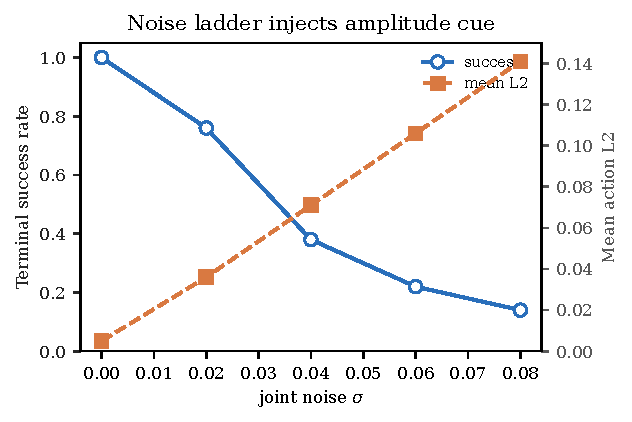
\includegraphics[width=0.98\linewidth]{figures/fig_noise_ladder.pdf}
\caption{Expert-perturbation CF couples failure with amplitude.}
\label{fig:ladder}
\end{figure}

\subsection{Q2: Does a WAM-style head fall for it---and recover?}
\label{sec:q2}

\begin{table*}[t]
\centering
\caption{\textbf{Dual-recipe decision and policy-update loops.} Direct rows use
argmax over scalar-matched directions ($n{=}120$ layouts/seed). Policy rows
distill feedback into identical policies on a disjoint update split and execute
without the evaluator
($n$ as listed). Entries are mean$\pm$std over five seeds.}
\label{tab:master}
\setlength{\tabcolsep}{3.5pt}
\renewcommand{\arraystretch}{1.08}
\resizebox{\textwidth}{!}{%
\begin{tabular}{@{}llcccc@{}}
\toprule
\rowcolor{hdr}
Family & Observation
  & Pert CL$\downarrow$
  & Paired CL$\uparrow$
  & Gap$\uparrow$
  & Runs \\
\midrule
\rowcolor{goodrow}
MiniWAM & privileged seats
  & $0.328{\pm}0.035$ & $\mathbf{0.973{\pm}0.009}$ & $\mathbf{0.645{\pm}0.036}$ & $n{=}120{\times}5$ \\
\rowcolor{goodrow}
MiniWAM & RGB centroids
  & $0.328{\pm}0.035$ & $\mathbf{0.948{\pm}0.041}$ & $\mathbf{0.620{\pm}0.066}$ & $n{=}120{\times}5$ \\
\rowcolor{goodrow}
MiniWAM & frozen DINOv2
  & $0.328{\pm}0.035$ & $\mathbf{0.947{\pm}0.015}$ & $\mathbf{0.618{\pm}0.044}$ & $n{=}120{\times}5$ \\
\rowcolor{goodrow}
FACT-style WAM (2.3M) & privileged seats
  & $0.330{\pm}0.032$ & $\mathbf{0.973{\pm}0.009}$ & $\mathbf{0.643{\pm}0.033}$ & $n{=}120{\times}5$ \\
\midrule
\rowcolor{goodrow}
Evaluator$\rightarrow$policy & privileged; evaluator-free test
  & $0.296{\pm}0.046$ & $\mathbf{0.976{\pm}0.012}$ & $\mathbf{0.680{\pm}0.040}$ & $n{=}90{\times}5$ \\
\rowcolor{goodrow}
Evaluator$\rightarrow$policy & frozen DINOv2; BC init.; RGB test
  & $0.565{\pm}0.136$ & $\mathbf{0.925{\pm}0.017}$ & $\mathbf{0.360{\pm}0.125}$ & $n{=}120{\times}5$ \\
\rowcolor{goodrow}
Evaluator$\rightarrow$policy & dynamic push
  & $0.271{\pm}0.094$ & $\mathbf{0.993{\pm}0.010}$ & $\mathbf{0.722{\pm}0.101}$ & $n{=}90{\times}5$ \\
\rowcolor{goodrow}
Evaluator$\rightarrow$policy & dynamic carry-release
  & $0.349{\pm}0.032$ & $\mathbf{1.000{\pm}0.000}$ & $\mathbf{0.651{\pm}0.032}$ & $n{=}90{\times}5$ \\
\bottomrule
\multicolumn{6}{@{}l@{}}{\footnotesize
Within each comparison, architecture, update rule, and held-out candidates are
fixed; training cardinality is reported and stressed separately below.}\\
\end{tabular}%
}
\end{table*}

\begin{figure}[t]
\centering
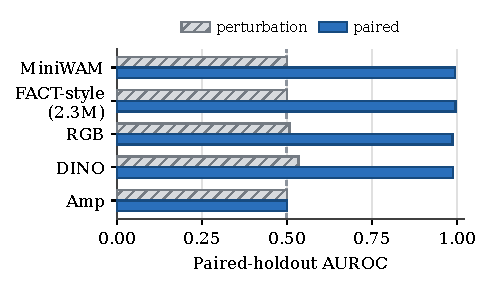
\includegraphics[width=\linewidth]{figures/fig_main_ranking.pdf}
\caption{\textbf{Paired-holdout ranking.} With the same heads, paired-geometry
training recovers near-perfect AUROC while perturbation training collapses.}
\label{fig:main_ranking}
\end{figure}

\begin{figure}[t]
\centering
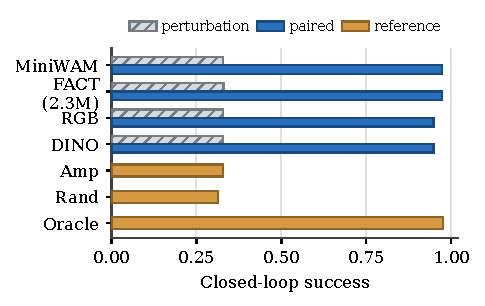
\includegraphics[width=\linewidth]{figures/fig_main_decision.pdf}
\caption{\textbf{Closed-loop selection.} Paired-geometry training approaches
the oracle; perturbation training collapses toward amplitude/random references.}
\label{fig:main_decision}
\end{figure}

Table~\ref{tab:master} is the decision-level contrast: same layouts, same
closed-loop rule, only the collection recipe changes.
Figs.~\ref{fig:main_ranking}--\ref{fig:main_decision} separate ranking quality
from its decision consequence. Under a shared large-$n$ protocol (5 seeds,
$n{=}120$),
MiniWAM seats / RGB / frozen DINOv2 and a FACT-style progress/value
Transformer (2.3M) all show the \emph{same qualitative} pattern---pert.\ CL
${\approx}0.33$, paired CL ${\approx}0.95$--$0.97$, gap ${\approx}0.62$--$0.65$---with
seed-level scatter that is not a copied row. Capacity does not erase the leak;
the FACT-style head does not claim parity with FACT's released video WAM. The
collapse is also not a logistic artifact: a scaled joint head on paired labels
still only reaches $0.389$.

\textbf{Policy improvement.}
We next freeze each evaluator, score the same matched candidate bank on a
layout-disjoint update split, and distill its temperature-scaled preferences
into identical geometry-conditioned policies. At test time the evaluator is
absent. For the RGB study, evaluator, eight-layout BC initialization, feedback
update, and test layouts are mutually disjoint; all updates use the same
$\mathrm{KL}{=}0.1$ anchor to the BC policy. We selected the smallest competent
BC budget on development seed~0; all reported RGB statistics use untouched
seeds~1--5. Across five seeds and 450 held-out layouts, no update reaches
$0.340{\pm}0.052$, confounded feedback reaches $0.296{\pm}0.046$, paired
feedback reaches $0.976{\pm}0.012$, and oracle feedback reaches
$0.969{\pm}0.020$. Paired minus confounded is $0.680{\pm}0.040$ (seed-bootstrap
95\% CI $[0.644,0.704]$; 5/5 positive). Thus confounded feedback does not improve
the proposal policy, whereas paired feedback transfers the recovered geometry
dependence into its parameters rather than relying on test-time reranking.
The same test is stronger under contact. Velocity-controlled push with randomized
mass/friction gives $0.271{\pm}0.094$ vs $0.993{\pm}0.010$ (pooled layout-bootstrap
gain CI $[0.680,0.764]$). Carry-release gives $0.349{\pm}0.032$ vs
$1.000{\pm}0.000$ (CI $[0.607,0.696]$). Its confounded policy learns the partial
lesson ``do not release early''---drop falls to zero---but $65.1\%$ of executions
still reach a wrong target. Paired feedback supplies the missing action--target
interaction, converting that semantic failure into correct placement (5/5 seeds).
Finally, replacing coordinates with frozen DINOv2 RGB features and initializing
all policies from the same eight-layout BC split gives no-update success
$0.645{\pm}0.154$, confounded-feedback success $0.565{\pm}0.136$, and
paired-feedback success $0.925{\pm}0.017$ on clean held-out images. Paired
feedback therefore improves an already competent policy by $0.280$ (pooled
layout-bootstrap CI $[0.245,0.317]$), whereas the confounded update is worse
than no update. Identical augmentation during policy distillation retains
paired success $0.882$ under Gaussian noise, $0.955$ under blur, $0.838$ under
rectangular occlusion, $0.923$ under crop, and $0.905$ under channel
permutation; the paired-minus-no-update CI is positive in every condition and
all five seeds are positive. The evaluator is absent in every reported
execution.

\begin{table*}[t]
\centering
\caption{Transfer and capacity controls. The same evaluation layouts are used
throughout; only the training recipe, feature source, or model width changes.}
\label{tab:q2_controls}
\setlength{\tabcolsep}{4pt}
\begin{tabular}{@{}lccc@{\qquad}lcccc@{}}
\toprule
\multicolumn{4}{c}{\textbf{(a) Full train$\times$eval transfer}} &
\multicolumn{4}{c}{\textbf{(b) Controls that preserve the gap}}\\
\rowcolor{hdr}
Train $\backslash$ Eval & Conf. AUROC & Paired AUROC & Paired CL &
Control & Conf. amp & Pert. CL & Paired CL / Gap \\
\midrule
Amp $\leftarrow$ conf. & 0.884 & 0.486 & 0.222 & Scale-up (150/240) & 0.909 & 0.347 & 0.972 / 0.625 \\
Scaled joint $\leftarrow$ paired & 0.512 & 0.522 & 0.389 & Joint-noise CF & 0.896 & 0.271 & 0.979 / 0.708 \\
MiniWAM $\leftarrow$ conf. & 1.000 & 0.500 & 0.250 & Gripper-delay CF & 0.931 & 0.271 & 0.979 / 0.708 \\
\rowcolor{goodrow}
MiniWAM $\leftarrow$ paired & 0.381 & \textbf{0.983} & \textbf{0.972} & Width $64{\rightarrow}512$ & --- & 0.313 & 1.000 / 0.688 \\
\midrule
Oracle / Random / Amp-heur. & --- & --- & 1.00 / 0.33 / 0.22 & & & & \\
\bottomrule
\end{tabular}
\end{table*}

Table~\ref{tab:q2_controls} fills every transfer cell: confounded training looks
perfect in-domain and collapses under amplitude control; paired MiniWAM is the
only recipe that both ranks and decides correctly. A scaled logistic joint head
trained on paired data reaches CL only~$0.389$---nonlinear fusion helps, but
protocol dominates. Across five seeds the MiniWAM gap is
$0.65\pm0.10$ (paired AUROC $0.993\pm0.006$, CL $0.950\pm0.036$).

\subsection{Controls: scale, capacity, and sample size}
\label{sec:robust}

\begin{figure}[t]
\centering
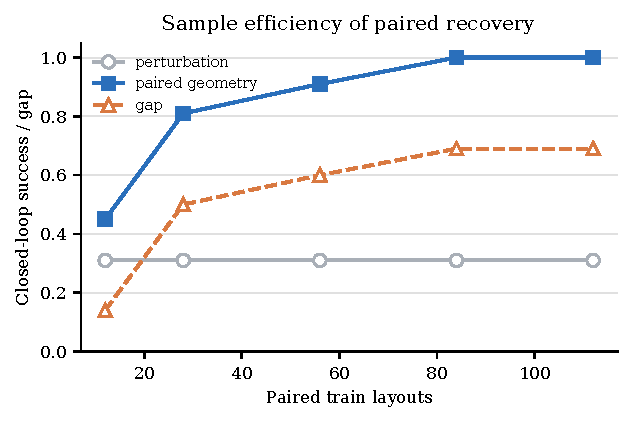
\includegraphics[width=0.98\linewidth]{figures/fig_sample_curve.pdf}
\caption{Paired recovery is data-efficient (gap vs.\ \#paired layouts).}
\label{fig:sample}
\end{figure}

Table~\ref{tab:q2_controls} compresses the non-story: larger splits, alternate CF
(joint noise or gripper delay), and a width sweep all preserve the
same qualitative gap---consistent with a \emph{label} confound, not
underfitting or a tiny-split artifact. Fig.~\ref{fig:sample} shows paired
recovery is cheap: gap~$0.50$ already at 28 layouts, plateauing near~$0.69$.
Keeping two of three matched directions per training layout cuts rollout cells
by $33\%$, while evaluation uses the full grid. At 28/56/112 layouts, sparse
CL is $0.886/0.989/1.000$ versus $0.979/1.000/1.000$ full (five seeds): cost is
visible only at the lowest data regime. With 5/7 directions, random CL falls to
$0.24/0.29$ while oracle CL stays $0.94/0.96$.

\subsection{Q3: Transfer---tasks, engines, vision}
\label{sec:q3}

\begin{figure*}[t]
\centering
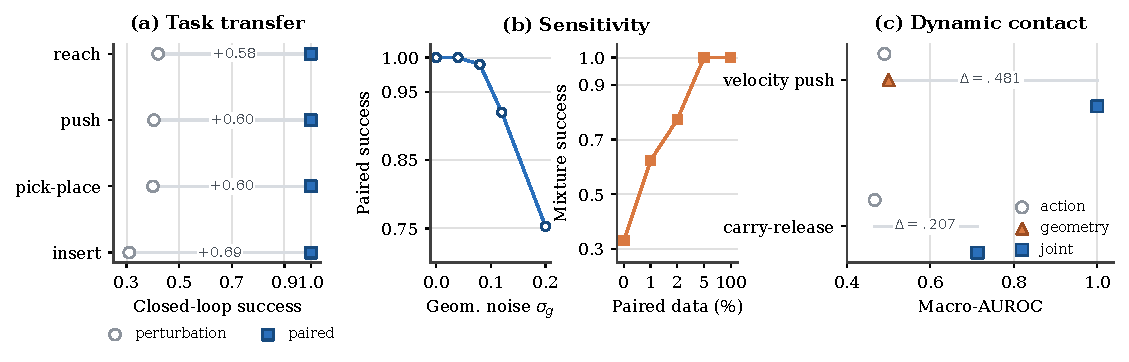
\includegraphics[width=0.98\textwidth]{figures/fig_transfer_robustness.pdf}
\caption{\textbf{Transfer and robustness.} (a)~Recipe gaps across tasks.
(b)~Geometry-noise and paired-data sensitivity. (c)~Dynamic-contact AUROC;
$\Delta$ is joint minus action (95\% CI). Five-seed means.}
\label{fig:q3_robustness}
\end{figure*}

Fig.~\ref{fig:q3_robustness}a shows perturbation CL at $0.31$--$0.42$ versus
paired CL $1.00$ on four tasks. Removing label leakage does not solve visual
optimization: paired/perturbation AUROC is $0.533/0.487$ (CNN),
$0.493/0.488$ (ResNet18), and $0.986/0.550$ (frozen DINOv2).
MuJoCo~\cite{todorov2012mujoco}, PyBullet~\cite{coumans2021pybullet}, and
SAPIEN~\cite{xiang2020sapien} match by design under the shared kinematic
contract (gap~$0.620$), excluding an API artifact rather than proving physics
transfer. Cross-task evaluation without task IDs preserves paired CL~$1.00$.
In Fig.~\ref{fig:q3_robustness}b, geometry noise produces a smooth
$1.00{\rightarrow}0.75$ decline, while ${\approx}5\%$ paired data saturates the
mixture curve. Continuous target jitter plus $6$--$10$~mm endpoint noise retains
a $0.37$--$0.48$ joint-minus-action macro-AUROC gain (600 rows/engine).

For contact-rich controls (Fig.~\ref{fig:q3_robustness}c), randomized
mass/friction push gains $0.481$ (CI $[0.411,0.568]$); three-outcome
carry-release gains $0.207$ ($[0.171,0.236]$). Every seed is positive. These are
predictor metrics; Table~\ref{tab:master} tests evaluator-free policy updates.

\begin{figure}[t]
\centering
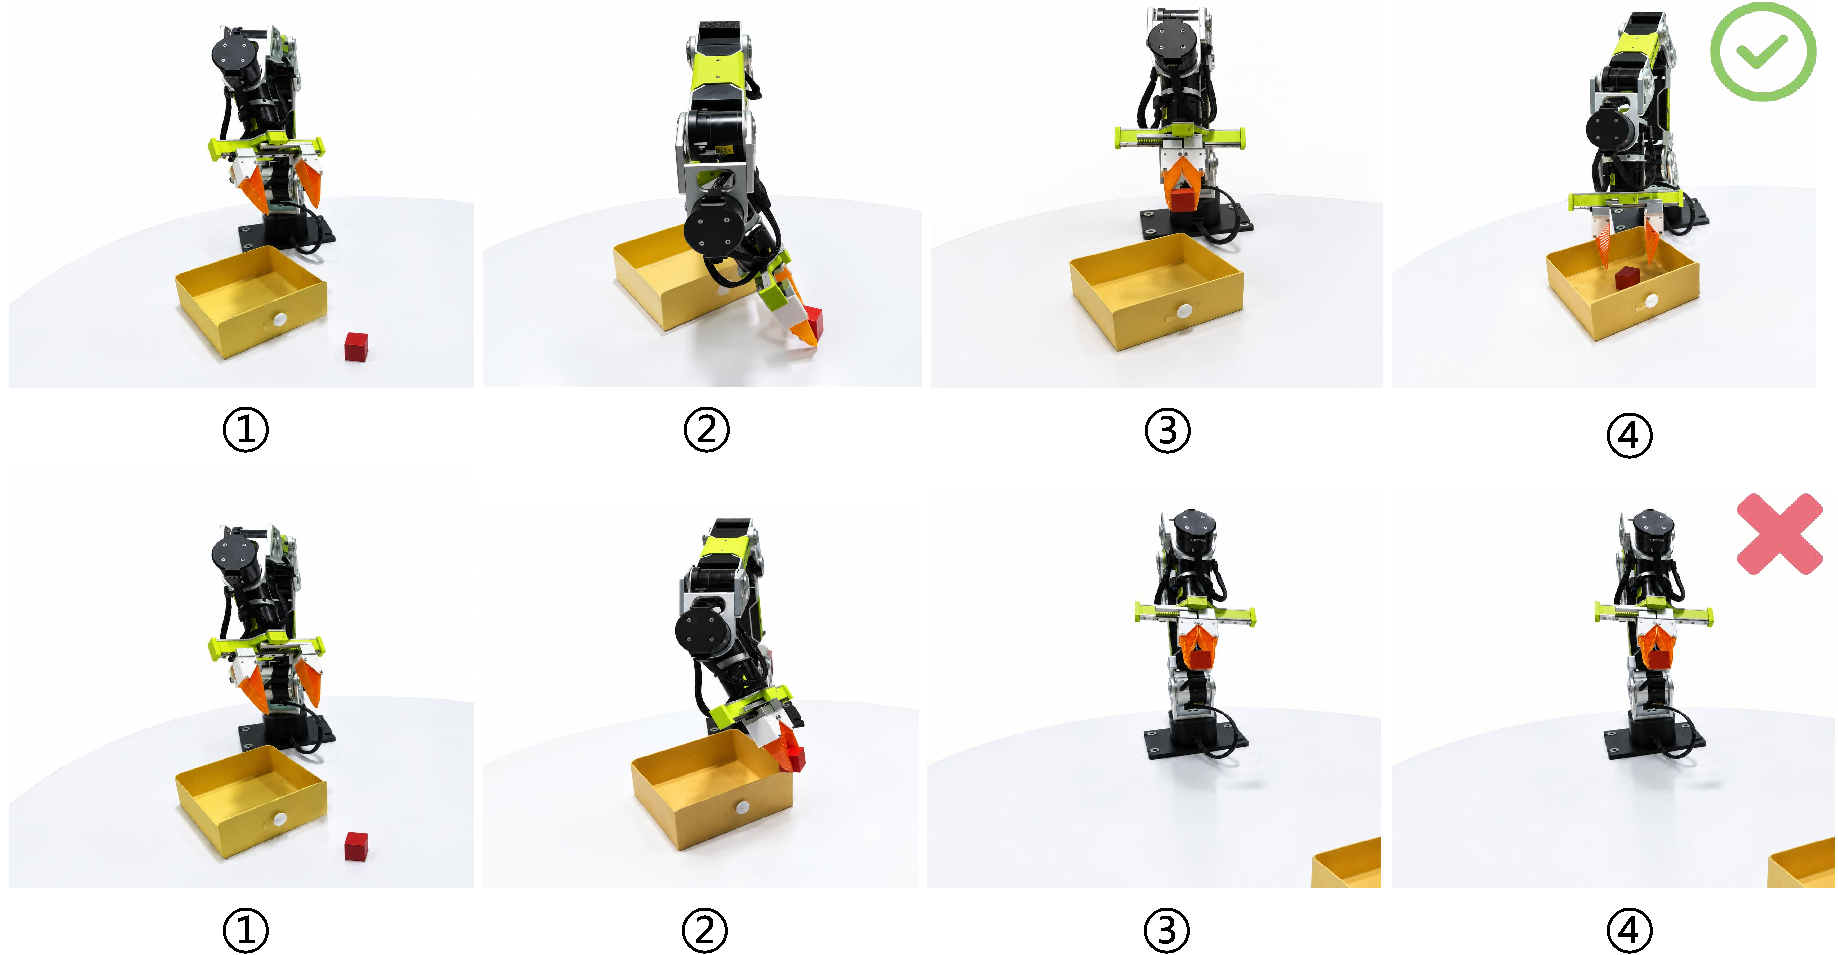
\includegraphics[width=\linewidth]{figures/fig_real.pdf}
\caption{\textbf{Representative real-tabletop executions.}
Top: successful red-cube pick-and-place. Bottom: placement failure.
This is qualitative physical evidence; quantitative paired-intervention
results remain simulation based.}
\label{fig:real_robot}
\end{figure}

\subsection{External real-video label audit}
\label{sec:public_audit}

We tested whether a bounded BridgeData V2~\cite{bridgedata2023} LeRobot shard
could support an external outcome audit. It cannot: no common success label is
present. Before fitting any model, two blinded raters judged 120 shared clips
drawn from 26 task strings and agreed perfectly ($\kappa{=}1.00$). An
endpoint-progress proxy agreed with that rater consensus on only $52.5\%$
(95\% CI $[43.3,61.7]\%$; balanced accuracy $41.3\%$); 113/120 clips showed
visible progress. We therefore
reject the proxy and withhold all public-data outcome/amplitude AUROC claims.
The shard, matching code, and negative audit remain in the artifact. BridgeData,
DROID~\cite{khazatsky2024droid}, or any expert-heavy collection must establish
verified outcome variation before a failure-shortcut audit is interpretable.

\subsection{Q4: Are failure data toxic---or unmatched amplitude?}
\label{sec:q4}

\begin{table}[t]
\centering
\caption{Failure data are not intrinsically toxic---unmatched amplitude is.}
\label{tab:fact}
\begin{tabular}{lcc}
\toprule
\rowcolor{hdr}
Recipe & Amp$\rightarrow$success AUROC \\
\midrule
Expert-perturbation CF (victim) & 0.90 \\
FACT-style matched-amp failures & 0.54 \\
Same fails mixed with larger moves & 1.00 \\
Frozen FACT / PointWorld on our obs & $\approx 0.51$ \\
\bottomrule
\end{tabular}
\end{table}

Table~\ref{tab:fact} separates toxicity from amplitude matching. FACT-style
matched-amplitude policy failures stay near chance (AUROC~$0.54$); mixing larger
failed moves with expert successes recreates AUROC~$1.00$. Frozen PointWorld
and FACT value probes on our synthetic observations stay near chance
($\approx 0.51$). We did not train public weights on the victim chain; AGCD
targets the \emph{wiring}, not an accusation that every release already leaks.

\section{Discussion}
\label{sec:disc}

\paragraph{Protocol before loss.}
A regularizer can suppress a representation of a confound that remains in the
labels. Paired geometry removes that cue at collection time, so AGCD is
upstream of representation learning: it gates failure-driven policy updates by
requiring (i) recipe amplitude AUROC, (ii) amplitude-controlled paired AUROC,
and (iii) closed-loop selection against an amplitude heuristic. Failure data are
useful only after this ranking test; the frozen FACT/PointWorld probes and the
public-video audit are controls, not claims that every released WAM is flawed.
This distinction matters for self-improvement: a failure trajectory can teach a
world model about consequences while still being an invalid target for an
outcome head if its label is predictable from perturbation size.

\paragraph{Decision consequence.}
The paired protocol is therefore a data-to-decision gate, not a new backbone or
loss. Once the joint head passes the crossing test, its score can be used for
candidate ranking, rejection, or evaluator-guided policy updates. If it fails,
additional capacity or calibration cannot recover the missing action--geometry
signal; the collection recipe must change first.

\paragraph{Why calibration is downstream.}
Temperature scaling preserves candidate ordering, while conformal rejection can
reduce coverage without removing a shortcut from accepted actions. Neither
creates geometry dependence when amplitude already reveals the label. AGCD
therefore tests paired ranking and execution before calibrating selective risk;
the reverse order can yield calibrated scores with physically wrong choices.

\paragraph{Cost and scaling.}
A complete $m\!\times\!n$ crossing is deliberately diagnostic rather than a
proposal to densely tile a continuous action space. Its purpose is to expose
identifiability before expensive training. Sparse matched directions reduce
collection by one third with little loss except at the smallest regime
(Sec.~\ref{sec:robust}). In higher dimensions, stratified matching and calipers
reduce cost, but change the claim from randomized counterfactual evidence to
observational evidence.

\paragraph{Scope and reproducibility.}
The main evidence is the MuJoCo FactorTask, with dynamic-contact and
cross-engine stress tests. RGB/DINO inputs use controlled visual markers, and
the BridgeData result is deliberately a negative proxy audit; neither implies
sim-to-real transfer. The release contains the factor generator, JSON gate
reports, model/task scripts, and tests; no checkpoint is needed to reproduce the
diagnostic. Fig.~\ref{fig:real_robot} documents the physical setup and outcome
contrast; exact paired interventions on hardware remain the next validation
step and do not change the paper's primary claim.

\paragraph{Physical validation protocol.}
The hardware study will preserve the diagnostic contrast rather than report
isolated successful grasps: scalar-matched candidates are replayed across
object layouts, Action-only and joint scores rank the same candidates, and
outcomes record grasp success, wrong-object/contact events, and rejection.
This small-scale test asks whether visible geometry changes real decisions; it
does not serve as a broad manipulation benchmark. Controlled tabletop resets
support the strongest comparison; if reset error cannot be bounded, results
will be reported as matched trials rather than exact counterfactuals.

\section{Conclusion}
\label{sec:conclusion}

Expert perturbations can inject an action-amplitude shortcut into outcome heads.
AGCD audits that recipe, holds action scalars fixed while varying geometry,
retrains the same head, and tests both selection and policy improvement. The
confounded predictor fails both; paired feedback restores ranking and transfers
to an evaluator-free policy. AGCD is a falsifiable data-to-decision-to-learning
contract for failure-driven WAMs, not a new backbone.

\bibliographystyle{IEEEtran}
\begin{thebibliography}{40}
\bibitem{ha2018recurrent} D.~Ha and J.~Schmidhuber, ``Recurrent world models
facilitate policy evolution,'' \emph{NeurIPS}, 2018.
\bibitem{hafner2025mastering} D.~Hafner et al., ``Mastering diverse control
tasks through world models,'' \emph{Nature}, 2025.
\bibitem{coco2026} Y.~Shi et al., ``Overcoming statistical bias in
action-controllable world models,'' arXiv:2608.04653, 2026.
\bibitem{fact2026} Q.~Peng et al., ``FACT: Failure-aware causal training for
world-action models,'' arXiv:2608.10232, 2026.
\bibitem{motus2_2026} H.~Bi et al., ``Motus2: A self-evolving general world
model for dexterous manipulation,'' arXiv:2608.30237, 2026.
\bibitem{flare2026} G.~Zhao et al., ``FLARE: A failure-aware framework for
autonomous correction and recovery in visual-language robotic manipulation,''
arXiv:2608.26645, 2026.
\bibitem{rlbench2019} S.~James et al., ``RLBench: The robot learning benchmark
\& learning environment,'' \emph{IEEE RA-L}, 2020.
\bibitem{gwm2026} Y.~Zhao et al., ``GWM-VLA: Geometry-aware latent world
modeling for vision-language-action learning,'' arXiv:2608.07619, 2026.
\bibitem{vggtworld2026} X.~Sun et al., ``VGGT-World: Transforming VGGT into an
autoregressive geometry world model,'' arXiv:2603.12655, 2026.
\bibitem{vggtomega2026} J.~Wang et al., ``VGGT-$\Omega$,'' arXiv:2605.15195,
2026.
\bibitem{vggt4d2025} Y.~Hu et al., ``VGGT4D: Mining Motion Cues in Visual
Geometry Transformers for 4D Scene Reconstruction,'' arXiv:2511.19971, 2025.
\bibitem{actbench2024} H.~Arai et al., ``ACT-Bench: Towards action controllable
world models for autonomous driving,'' arXiv:2412.05337, 2024.
\bibitem{validate2026} C.~Oefinger et al., ``Validate the dream before you
trust its verdict,'' arXiv:2607.07196, 2026.
\bibitem{geirhos2020shortcut} R.~Geirhos et al., ``Shortcut learning in deep
neural networks,'' \emph{Nature Machine Intelligence}, 2020.
\bibitem{arjovsky2019irm} M.~Arjovsky et al., ``Invariant risk minimization,''
arXiv:1907.02893, 2019.
\bibitem{bridgedata2023} H.~Walke et al., ``BridgeData V2: A Dataset for Robot
Learning at Scale,'' \emph{CoRL}, 2023.
\bibitem{pointworld2026} W.~Huang, Y.-W.~Chao, A.~Mousavian, M.-Y.~Liu,
D.~Fox, K.~Mo, and L.~Fei-Fei, ``PointWorld: Scaling 3D world models for
in-the-wild robotic manipulation,'' arXiv:2601.03782, 2026.
\bibitem{chi2023diffusion} C.~Chi, Z.~Xu, S.~Feng, E.~Cousineau, Y.~Du,
B.~Burchfiel, R.~Tedrake, and S.~Song, ``Diffusion Policy: Visuomotor policy
learning via action diffusion,'' \emph{RSS}, 2023.
\bibitem{ross2011dagger} S.~Ross, G.~J.~Gordon, and J.~A.~Bagnell, ``A
reduction of imitation learning and structured prediction to no-regret online
learning,'' \emph{AISTATS}, 2011.
\bibitem{dehaan2019causal} P.~de Haan, D.~Jayaraman, and S.~Levine, ``Causal
confusion in imitation learning,'' \emph{NeurIPS}, 2019.
\bibitem{khazatsky2024droid} A.~Khazatsky et al., ``DROID: A large-scale
in-the-wild robot manipulation dataset,'' \emph{RSS}, 2024.
\bibitem{openx2024} Open X-Embodiment Collaboration et al., ``Open
X-Embodiment: Robotic learning datasets and RT-X models,'' \emph{ICRA}, 2024.
\bibitem{finn2016video} C.~Finn, I.~Goodfellow, and S.~Levine, ``Unsupervised
learning for physical interaction through video prediction,'' \emph{NeurIPS},
2016.
\bibitem{finn2017foresight} C.~Finn and S.~Levine, ``Deep visual foresight for
planning robot motion,'' \emph{ICRA}, 2017.
\bibitem{hafner2019planet} D.~Hafner, T.~Lillicrap, I.~Fischer, R.~Villegas,
D.~Ha, H.~Lee, and J.~Davidson, ``Learning latent dynamics for planning from
pixels,'' \emph{ICML}, 2019.
\bibitem{dasari2020robonet} S.~Dasari et al., ``RoboNet: Large-scale
multi-robot learning,'' \emph{CoRL}, 2020.
\bibitem{mandlekar2022robomimic} A.~Mandlekar et al., ``What matters in
learning from offline human demonstrations for robot manipulation,''
\emph{CoRL}, 2022.
\bibitem{liu2023libero} B.~Liu, Y.~Zhu, C.~Gao, Y.~Feng, Q.~Liu, Y.~Zhu, and
P.~Stone, ``LIBERO: Benchmarking knowledge transfer for lifelong robot
learning,'' \emph{NeurIPS Datasets and Benchmarks}, 2023.
\bibitem{mees2022calvin} O.~Mees, L.~Hermann, E.~Rosete-Beas, and W.~Burgard,
``CALVIN: A benchmark for language-conditioned policy learning for long-horizon
robot manipulation tasks,'' \emph{IEEE RA-L}, 2022.
\bibitem{guo2017calibration} C.~Guo, G.~Pleiss, Y.~Sun, and K.~Q.~Weinberger,
``On calibration of modern neural networks,'' \emph{ICML}, 2017.
\bibitem{geifman2019selective} Y.~Geifman and R.~El-Yaniv, ``SelectiveNet: A
deep neural network with an integrated reject option,'' \emph{ICML}, 2019.
\bibitem{angelopoulos2024crc} A.~N.~Angelopoulos, S.~Bates, A.~Fisch, L.~Lei,
and T.~Schuster, ``Conformal risk control,'' \emph{ICLR}, 2024.
\bibitem{oquab2024dinov2} M.~Oquab et al., ``DINOv2: Learning robust visual
features without supervision,'' \emph{TMLR}, 2024.
\bibitem{todorov2012mujoco} E.~Todorov, T.~Erez, and Y.~Tassa, ``MuJoCo: A
physics engine for model-based control,'' \emph{IROS}, 2012.
\bibitem{coumans2021pybullet} E.~Coumans and Y.~Bai, ``PyBullet, a Python
module for physics simulation for games, robotics and machine learning,''
2016--2021. [Online]. Available: https://pybullet.org
\bibitem{xiang2020sapien} F.~Xiang et al., ``SAPIEN: A SimulAted Part-Based
Interactive ENvironment,'' \emph{CVPR}, 2020.
\end{thebibliography}

\end{document}
